\section{Detección de marcadores}
Una vez realizada la captura de video del paciente, el primer paso en el procesamiento de las secuencias de video en un sistema de captura de movimiento es reconocer los marcadores en el cuerpo del sujeto, para luego tener la posición de cada uno de ellos en el espacio y a lo largo del tiempo.

Como se pudo ver anteriormente, para este sistema las condiciones de captura de las secuencias son muy favorables lo que permite utilizar métodos simples de segmentación basados en el estudio de los píxeles de la imagen.

El bloque de detección de marcadores, se puede dividir en dos partes bien definidas: la \textbf{segmentación} y el \textbf{filtrado de objetos} hasta obtener los marcadores. En la Figura \ref{ejemplotodointro} se muestra el resultado del procesamiento de cada parte.

\begin{figure}[ht!]
        \centering
        \subfloat[Captura original]{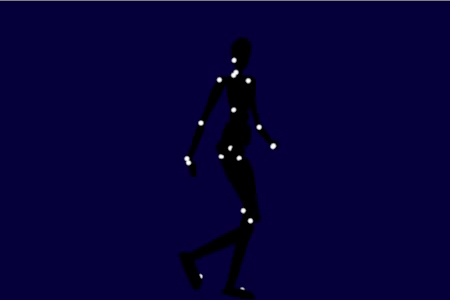
\includegraphics[scale=0.3]{imagenes/peladoFondoAzul.png} %\label{peladoOriginalintro}
        } \hspace{1cm}        
        \subfloat[Segmentación]{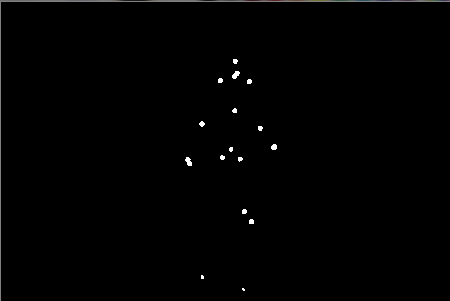
\includegraphics[scale=0.3]{imagenes/peladoFondoAzul_filtro.png}\label{peladoFiltrointro}}

        \subfloat[Detección]{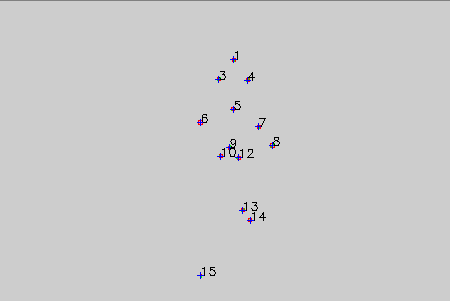
\includegraphics[scale=0.3]{imagenes/peladoFondoAzul_circulos.png} %\label{peladocirculosintro}
        }
  \caption{Ejemplo de funcionamiento del bloque.}
      \label{ejemplotodointro}
\end{figure}

\subsection{Segmentación}
En lo que respecta al bloque de segmentación, existen muchos métodos para implementar el mismo. Se comenzaron probando los más simples y se fue aumentando el nivel de complejidad hasta encontrar un método que se ajuste a los requerimientos del sistema. Finalmente, se eligió utilizar la umbralización, generando umbrales con el método de Otsu\cite{otsu} de tres clases.

Con el método de Otsu \cite{otsu} se pretende, a partir del histograma de la imagen, separar los píxeles de dicha imagen en tres niveles encontrando dos umbrales que los separen. Trabajar con tres clases permite ser un poco más flexible con los contrastes entre los marcadores y el resto de la imagen por lo que no sería estrictamente necesario, por ejemplo, que el traje del paciente y el fondo sean del mismo color.

\begin{figure}[ht!]
        \hspace{-0.6cm}
        \subfloat[Original]{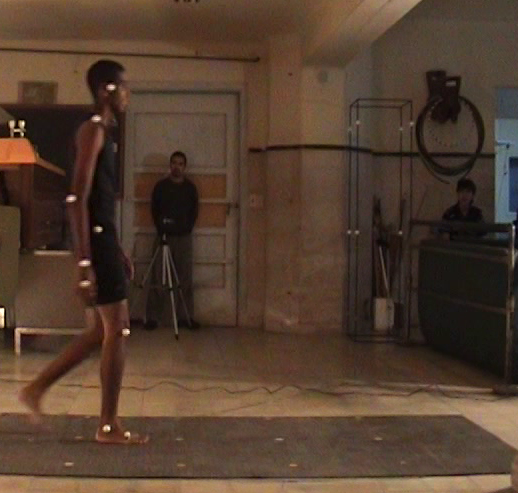
\includegraphics[scale=0.3]{imagenes/abel.png}\label{abelreal} 
         } \hspace{0.1cm}        
       \subfloat[Histograma]{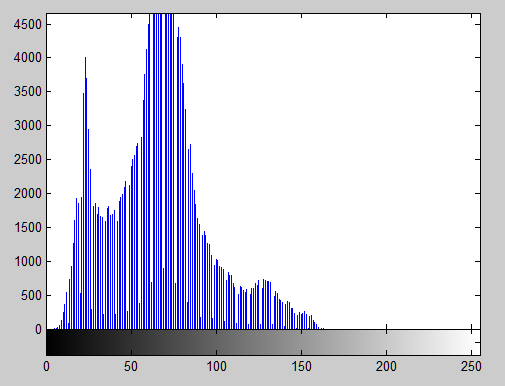
\includegraphics[scale=0.37]{imagenes/hist_abel.png}\label{histabel}}
  \caption{Captura original de un paciente real y su histograma de intensidad de pixeles.}
      \label{abelhistposta}
\end{figure}

En la Figura \ref{histabel} se observa el histograma de intensidad de píxeles de la imagen \ref{abelreal}, que corresponde a una captura de un paciente real. Dicho histograma muestra tres picos bien definidos, por lo que utilizar el método de Otsu de tres clases parece una buena opción para determinar los umbrales de segmentación. Manteniendo esta relación de intensidades entre fondo, ropa del paciente y marcadores, este método funcionaría adecuadamente para el bloque.


El bloque de segmentación de este sistema fue implementado en el lenguaje C++, debido a que es uno de los lenguajes de programación que cuenta con mayor cantidad de recursos para procesamiento de imágenes. En particular, se utilizaron las librerías \emph{OpenCV} \cite{opencv} y CVBlob \cite{cvblob} ya que funcionan para las plataformas principales de PC y dispositivos móviles, y están diseñadas para tener una gran eficiencia computacional en las implementaciones. Además, estas librerías son bastante populares dentro de las librerías de código abierto con similares características, lo cual implica que poseen una comunidad activa de usuarios muy grande.

\subsection{Filtrado}
 La etapa de filtrado de objetos no es más que una clasificación de los objetos segmentados. Dado que los objetos a detectar tienen formas relativamente sencillas (círculos blancos sobre fondo oscuro) y las condiciones de laboratorio son controladas al realizar la captura, esta etapa no requerirá implementar algoritmos muy complejos. En particular, se implementó un detector de objetos circulares en base a momentos geométricos y un filtro según el área de los mismos.